\documentclass[assignment01_Solutions]{subfiles}

\IfSubStr{\jobname}{\detokenize{Solutions}}{\toggletrue{solutions}}{\toggletrue{solutions}}

%\IfSubStr{\jobname}{\detokenize{Solutions}}{\toggletrue{solutions}}{\togglefalse{solutions}}

\fancypagestyle{firstpage}

{\rhead{Assignment 1 \linebreak \textit{Version: \today}}}

\title{Assignment 1: Linear Regression}
\author{Machine Learning}
\date{Fall 2019}

\begin{document}

\maketitle
\thispagestyle{firstpage}


\begin{learningobjectives}
\bi
\item Gain some familiarity with some of the key ideas in machine learning.
\item Review of mathematical concepts we will be using in the beginning part of this course.
\item Familiarizing yourself with computational toolset
\item Learn linear regression using a ``top-down'' approach.
\ei
\end{learningobjectives}


\begin{priorknowledge}
\bi
\item Basic machine learning terminology
\item Supervised learning problem framing
\ei
\end{priorknowledge}


\begin{recall}[Supervised Learning Problem Setup]
In the first class we saw the basic supervised learning problem setup.

Suppose you are given a training set of datapoints, $(\mlvec{x_1}, y_1), (\mlvec{x}_2, y_2), \ldots, (\mlvec{x}_n, y_n)$ where each $\mlvec{x_i}$ represents an element of an input space (e.g., a d-dimensional feature vector) and each $y_i$ represents an element of an output space (e.g., a scalar target value).  In the supervised learning setting, your goal is to determine a function $\hat{f}$ that maps from the input space to the output space.

We typically also assume that there is some loss function, $\ell$, that determines the amount of loss that a particular prediction $\hat{y}_i$ incurs due to a mismatch with the actual output $y_i$.  We can define the best possible model, $\hat{f}^\star$ as the one that minimizes these losses over the training set.  This notion can be expressed with the following equation  (note: that $\argmin$ in the equation below just means the value that minimizes the expression inside of the $\argmin$, e.g., $\argmin_{x} (x - 2)^2 = 2$, whereas $\min_{x} (x-2)^2 = 0$).
\begin{align}
\hat{f}^\star &= \argmin_{\hat{f}} \sum_{i=1}^n \ell \left ( \hat{f}(\mlvec{x_i}), y_i \right )
\end{align} 

\end{recall}



\section{Six Big Ideas in Machine Learning}
Before diving into the specifics of our first machine learning algorithm, let's examine some important ideas in machine learning.  Why six instead of seven?  if Rob Martello has taught us anything, it's that all good things come in sixes.%  For this set of six big ideas, we'll pay special attention to those that are most relevant to the module at hand (computer vision).


\subsection*{Idea 1: Correlations for the Win?}
ML algorithms learn to exploit correlations in data in order to make predictions.  For instance, if one was using a machine learning approach to learn to recognize smiles from images, the algorithm might determine that bright pixels around the mouth area of a face are correlated with smiling faces (e.g., they indicate that a person's teeth are showing).  This correlation would likely be useful for determining whether a new image of a face was a smile or not.  Unfortunately, while exploiting correlations is one of the most powerful aspects of ML systems, it is also one of the most potentially problematic aspects.


\bi

\item \emph{Example 1: Reinforcing Hiring Biases}
You likely heard the news that \href{https://www.reuters.com/article/us-amazon-com-jobs-automation-insight/amazon-scraps-secret-ai-recruiting-tool-that-showed-bias-against-women-idUSKCN1MK08G}{Amazon scrapped a secret AI recruiting tool that showed bias against women}.  More specifically, the tool performed automatic keyword analysis of job applications to predict whether or not the the applicant was worth forwarding on to a human evaluator for a closer look.  Early in the development of this system, researchers discovered that the model the system had learned placed a negative weight on words such as ``women's'' as well as the names of some women's colleges.  While there is of course no causal link between these words appearing in a job application and the suitability of the candidate for the job, there was a \emph{correlation} in the training set that was used to build the system between the presence of words such as ``women's'' and the candidates not being invited for interviews.

Why might such a correlation exist in the training set?  There are many different possible explanations for this correlation, ranging from overt or unconscious bias in the applicant evaluators whose judgments helped form the training data to systemic discrimination that denies women equal access to educational opportunities in STEM.  The important thing to take away from this is not that why there was a correlation, but that since the correlation existed in the training data the model learned to utilize that in order to evaluate new data.  Amazon realized that this was suboptimal and decided to take steps to address the problem (they say they never used the system to make actual job-screening decisions).  Despite efforts to prevent the algorithm for exploiting such correlations, the group determined that they couldn't fully guarantee that the algorithm had not found another way to achieve the same discriminatory outcome and terminated the project.


\item \emph{Example 2: Adversarial Machine Learning}

A second example of an ML algorithm exploiting correlations in training data in unexpected ways can be found in the field of of computer vision methods for object detection.  Identifying salient visual objects such as road signs and pedestrians is an important building block for applications such as autonomous driving.  A popular algorithm for this task, \href{https://pjreddie.com/darknet/yolo/}{YOLO} (You Only Look Once)\footnote{\href{https://www.youtube.com/watch?time_continue=77&v=MPU2HistivI}{Cool video of YOLO version 3}, \href{https://www.youtube.com/watch?v=Cgxsv1riJhI}{TED talk from the YOLO head researcher}}, can identify and localize objects in images with surprisingly good accuracy.  For instance, in the image below you can see how YOLO can be used to detect stop signs in an image.
\begin{center}
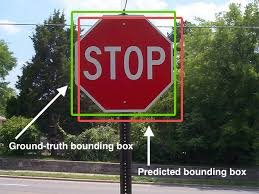
\includegraphics[width=0.6\linewidth]{figures/stopsignyolo}
\end{center}

While this all seems great, and YOLO achieves high accuracy at tasks such as this, there is a catch.  It is very difficult to understand \emph{how} YOLO is making these predictions.  That is, what is it about this image that causes the YOLO algorithm to be able to tell that it is a stop sign?  Perhaps it is the white text on the red background.  Perhaps it is the actual word ``STOP.''  The fact is that the network that makes this prediction is so complex, that is impossible for us to say definitively exactly how it makes its decision.

\begin{marginfigure}
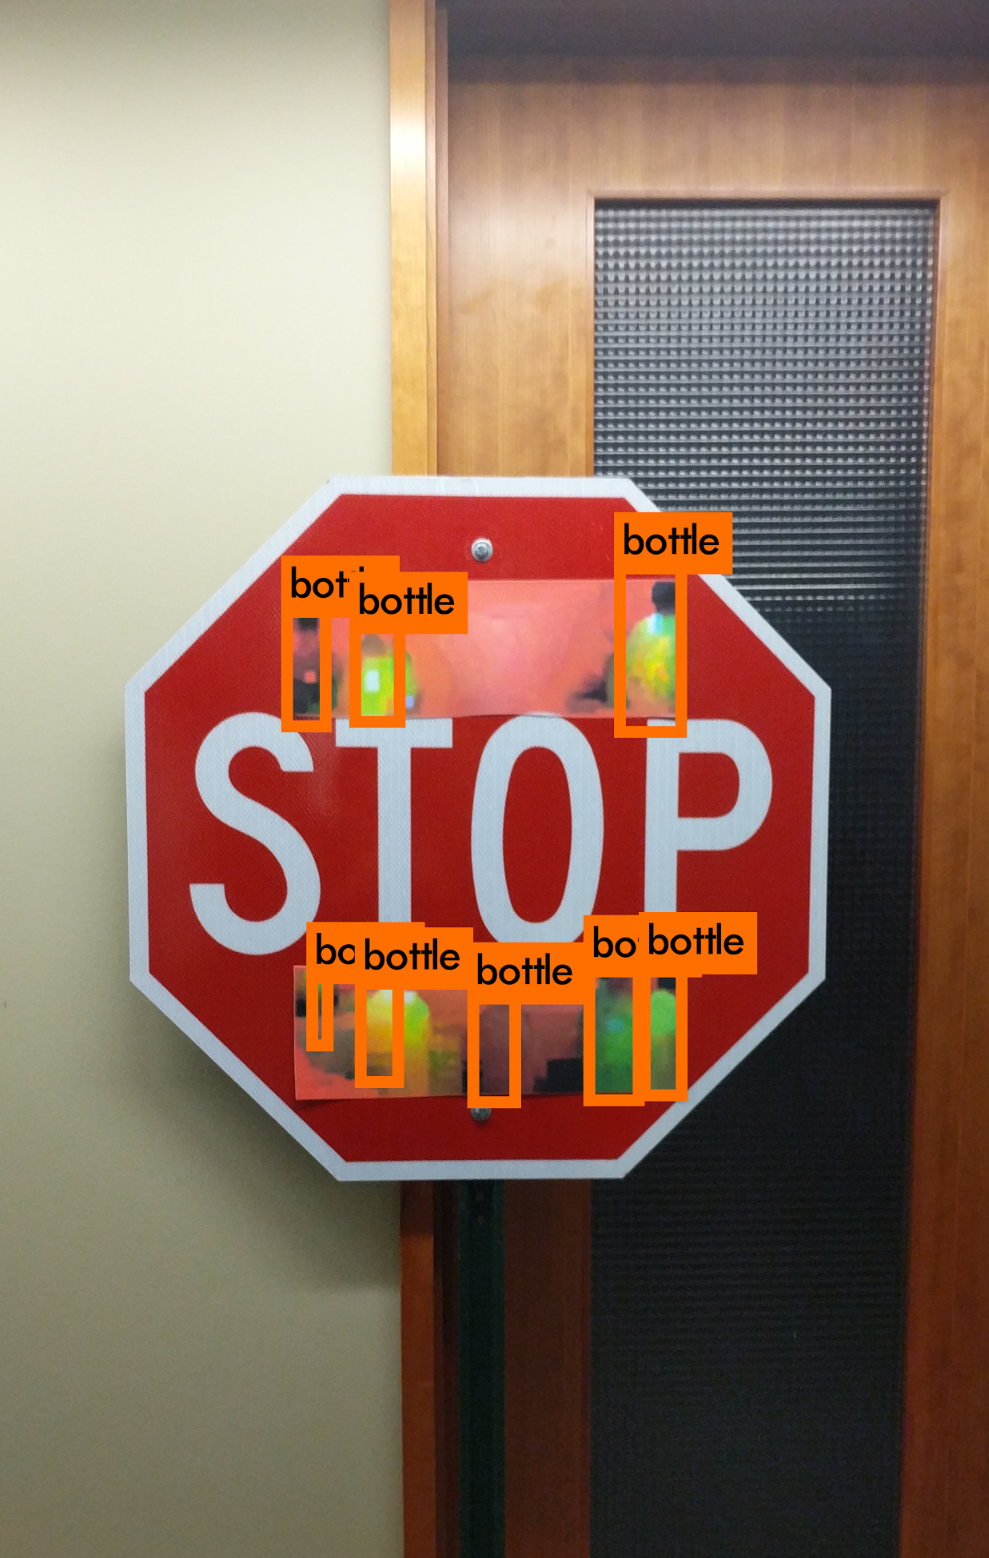
\includegraphics[width=1.6in]{figures/yolofooled}
\caption{A stop sign with a specially crafted sticker that causes a neural network to fail to identify it as as top sign.}\label{fig:yolofooled}
\end{marginfigure}
The complexity of the model makes it vulnerable to bad actors (or adversaries).  Researchers at University of Michigan used a form of ML known as \emph{adversarial machine learning} to \href{https://iotsecurity.engin.umich.edu/physical-adversarial-examples-for-object-detectors/}{create a specially crafted sticker that could be attached to a stop sign that would make it invisible to the YOLO model} (that is YOLO would not identify it as a stop sign).  Clearly, this has major implications for the safety of using a model such as this in an application like a self-driving car.   An example of the attach is shown in Figure~\ref{fig:yolofooled}.


\ei

\subsection*{Idea 2: There's No Such Thing as a Free Lunch}

\begin{quotation}
\href{https://en.wikipedia.org/wiki/All_models_are_wrong}{``All models are wrong, but some useful.''}

--- George Box
\end{quotation}

At the beginning of this document we have a reminder of the basic supervised machine learning setup.  At the most basic level, we try generalize from a set of training data to construct a function $\hat{f}^\star$ that best predicts the corresponding output data for unseen input data (e.g., predicting the facial expression of a face that was not in the training set based on a training set of sample faces and their corresponding expressions).  In the previous big idea, we discussed how machine learning could go wrong when there are correlations in the data that seem useful to the ML algorithm, but are ultimately counterproductive to how we'd like the system to make decisions.  It turns out that even before you choose the training for your algorithm, you must provide an \href{https://en.wikipedia.org/wiki/Inductive_bias}{inductive bias} to constrain the space of possible models you might fit.  Examples of common inductive biases include the following (the previously linked article has some more).
\be
\item The prediction function $\hat{f}^\star$ should smoothly change as you vary the input $\mlvec{x}$.
\item The prediction function has a particular form (e.g., linear).
\item The prediction function is sparse in that it ignores the majority of the inputs.
\ee

In fact, there are a whole class of theorems called \href{https://en.wikipedia.org/wiki/No_free_lunch_theorem}{No-Free-Lunch (NFL) theorems} that state that without inductive biases (such as the ones stated above), learning from data is essentially impossible.  This connects us back to the quote from George Box.  While the inductive bias we encode into our model will never be a fully represent reality, having this bias is necessary to allow the model to do the useful work of making predictions.  What's important for us as machine learning scientists and practitioners is to be explicit about the biases we are introducing when settling on a particular model so that we can best evaluate our results and predict the limitations of our systems.

\subsection*{Idea 3: It's All About How You Frame the Problem}
Using Machine Learning algorithms can be a bit disorienting for someone used to the typical engineering workflow.  A cartoon picture of the engineering workflow is that you are given a problem (perhaps it is initially difficult to solve or ambiguous), you might reframe the problem to make it easier to solve, and then you work to devise a solution to the reframed problem.  In machine learning, the last step is automated!  Your job as an ML practitioner is to reframe the original problem so that the ML algorithm can compute a solution.  If you've done the reframing properly, the solution to the reframed problem will also be a good solution to the original problem.

As an example, consider the use of a machine learning algorithm to teach a virtual character to walk in a simulated environment.  You might reframe this problem for the ML algorithm as tasking it with computing a controller for the virtual character that moves the character's center of mass forward as fast as possible.  The ML algorithm can now search over a vast space of possible control strategies to learn the one that most quickly propels the center of mass.  However, it doesn't necessarily follow that this controller will result in the character walking using a normal bipedal gait.

\begin{center}
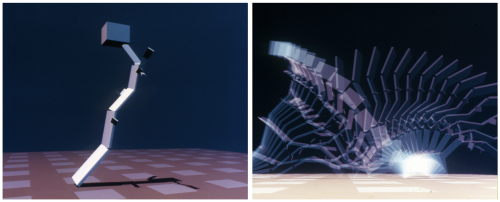
\includegraphics[width=.6\linewidth]{figures/fallingbot}
\end{center}

The notion that the solution an algorithm finds might be unpredictable to the designer is known as ``emergence.''  Some cool examples of this played out in actual experiments in evolving virtual creatures are summarized in the paper \href{https://arxiv.org/pdf/1803.03453.pdf}{The Surprising Creativity of Digital Evolution}.  For instance, a virtual character learned that falling down, see picture above, and getting up was more efficient for locomotion than constantly hopping (which is what the designer had intended the system to learn).

For more examples of this sort of thing, consider checking out \href{https://www.youtube.com/watch?v=bBt0imn77Zg}{Karl Sims: Evolved Virtual Creatures} or the short article \href{https://aiweirdness.com/post/172894792687/when-algorithms-surprise-us}{When AI Surprises Us}.  This also connects back to the age-old debate over whether \href{https://www.youtube.com/watch?v=8M_1GAX3WcI}{falling with style can be considered flying}.


\subsection*{Idea 4: ML Systems Can Learn Intermediate Representations}

In the next few weeks we'll learn about artificial neural networks (ANNs).  ANNs are biologically inspired algorithms since their functioning, at an abstract level, is modeled on the functioning of biological neurons (e.g., in the brain).

\begin{marginfigure}
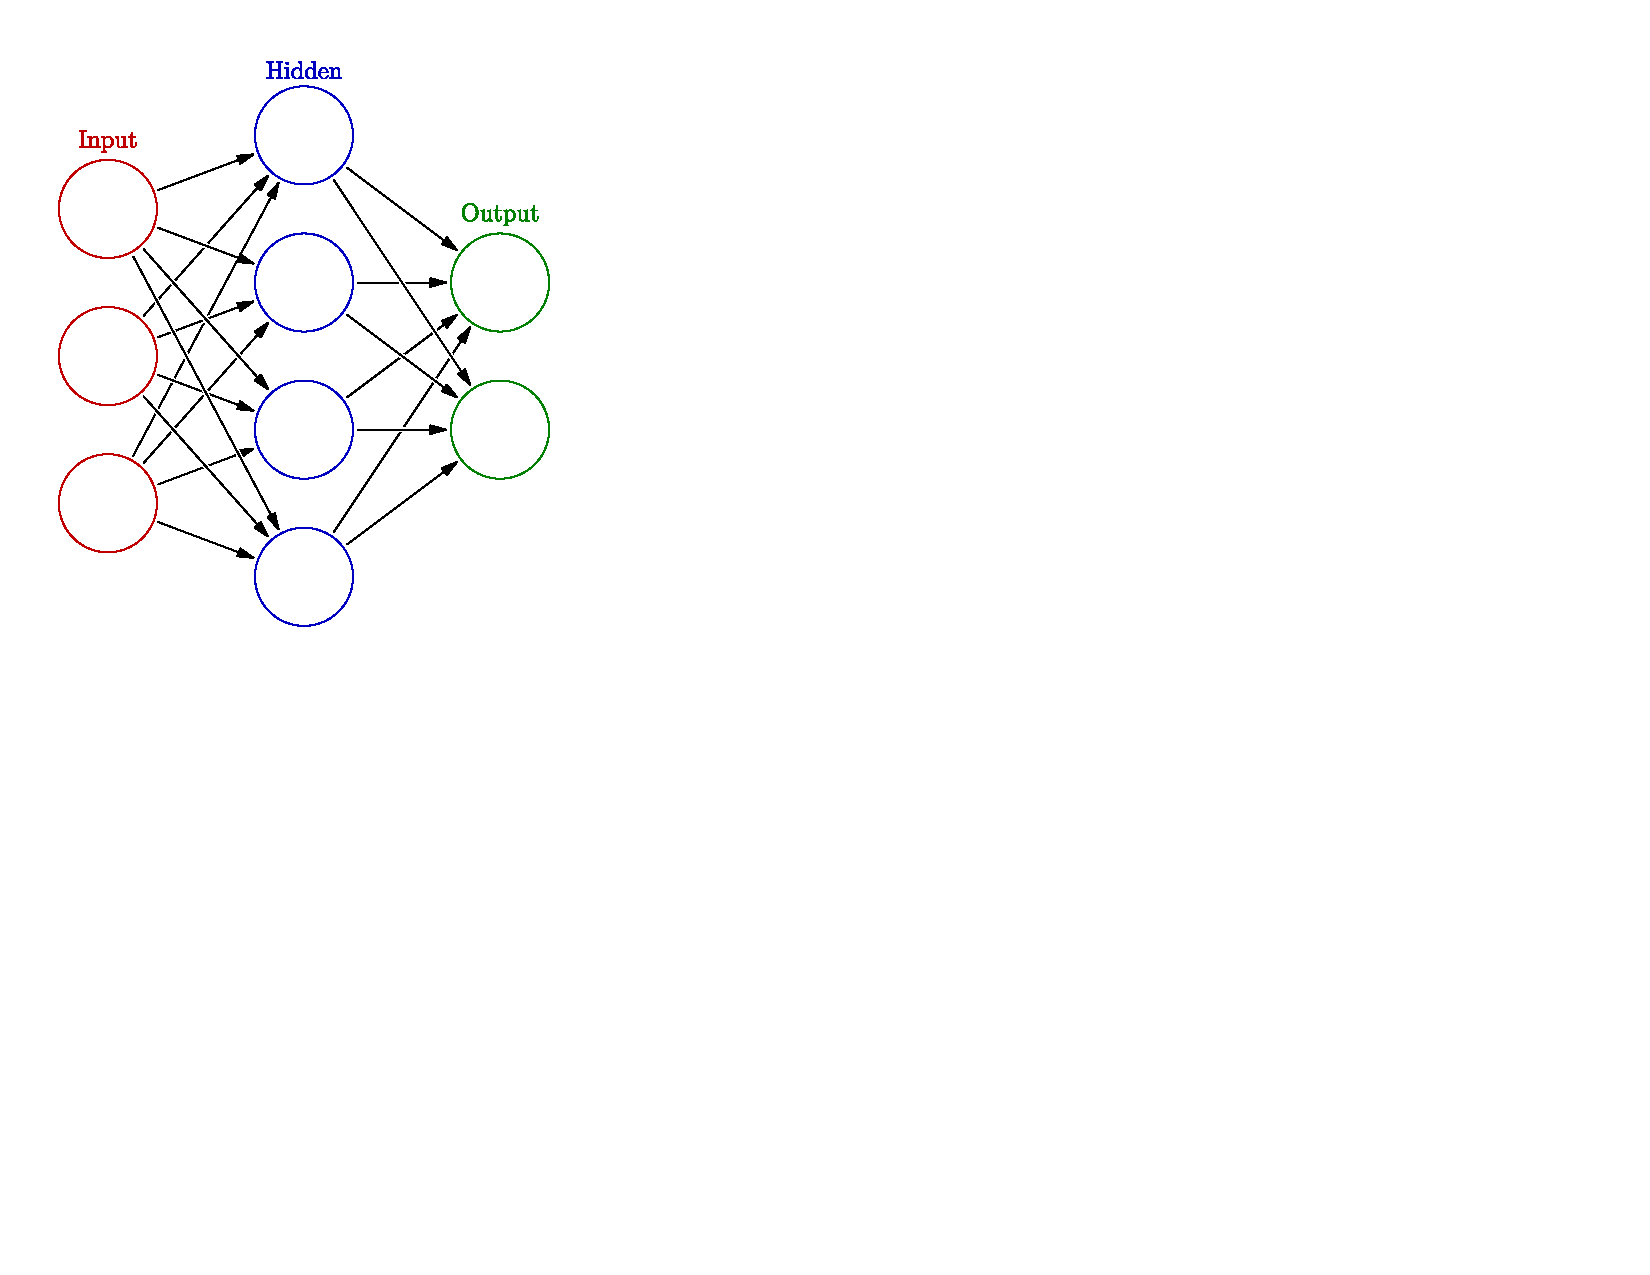
\includegraphics[width=1.8in]{figures/Colored_neural_network}
\caption{An artificial neural network with a single hidden layer.}\label{fig:ann}
\end{marginfigure}
ANNs accept input patterns at an array of virtual neurons called the input layer (see Figure~\ref{fig:ann}).  The neurons in the input layer are connected to other neurons via virtual axons that control to what extent a particular input neuron activates a downstream neuron.  The second set of neurons, called the ``hidden layer'' (shown in blue in the figure), is responsible for computing intermediate, hidden representations of the input data.  This process continues as activations propagate through the network until activations are generated at the output layer (shown in green). These outputs could correspond to any salient properties of the input (e.g., if the input is an image, the output might encode the objects in the image).

What's amazing about ANNs is that there are learning algorithms for setting the connections strengths between these virtual neurons (the black arrows in the figure) based on training data (input / output pairs).  These learning algorithms tune the connections strengths (also called ``weights'') such that for the provided training data, the network produces the appropriate training outputs (e.g., if you show the network a training set of images of cats or dogs, over time the network will adjust its weights so that the output says ``cat'' when presented an image of a cat and ``dog'' if presented an image of a dog).  The algorithms used to tune the network weights are only concerned with reproducing the output patterns, the network is free to choose how it represents information within the network (i.e., at the hidden layer).

\begin{marginfigure}

\caption{12x12 receptive fields learned from an neural network trained to optimally compress images}
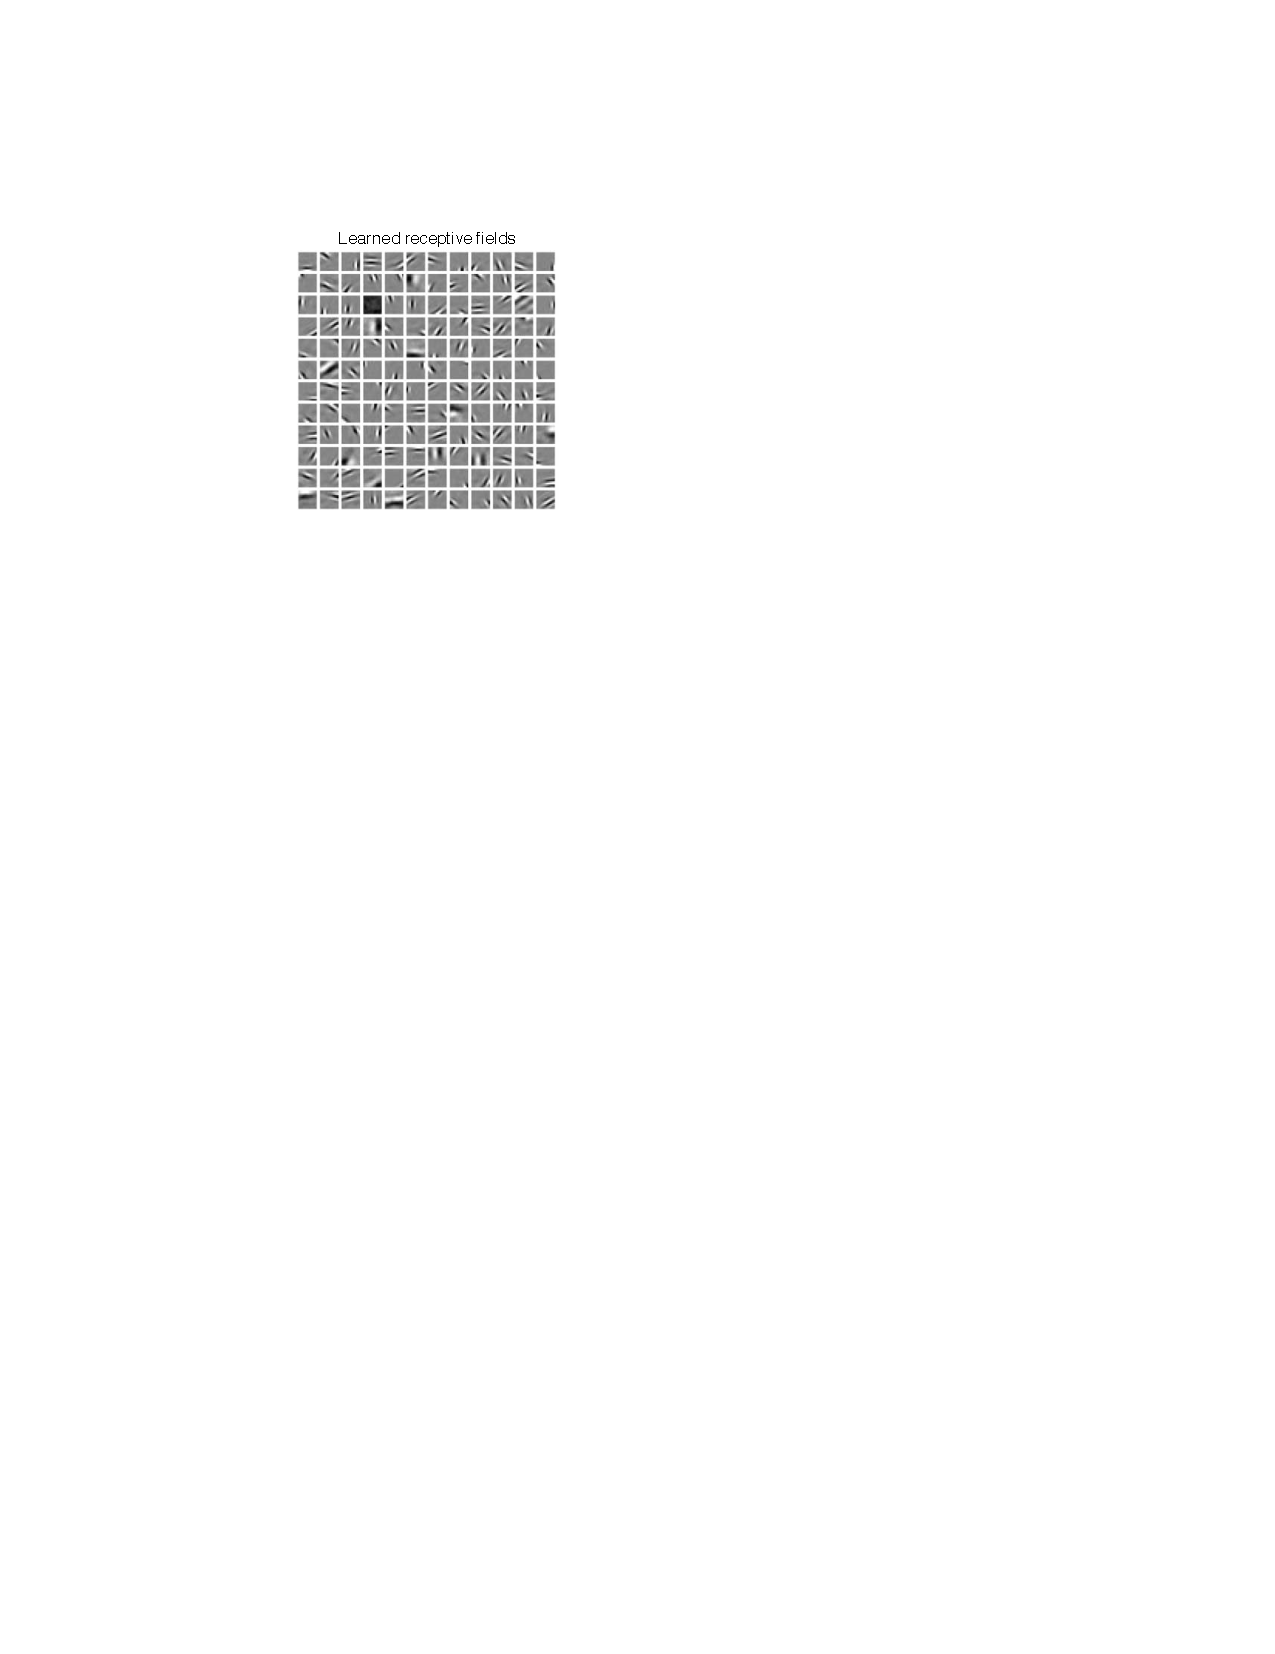
\includegraphics[width=1.5in]{figures/learned_receptive_fields}\label{fig:learnedfields}
\end{marginfigure}
What's super amazing is that we can actually examine the internal representations of a neural network to understand how it's performing the computation from input to output. For instance, Figure~\ref{fig:learnedfields}\footnote{From \href{http://www.cnbc.cmu.edu/~tai/nc19journalclubs/Olshausen-Field-CON-2004-1.pdf}{Sparse coding of sensory inputs}} shows a visualization of the internal representations learned by a network trained to best compress a training set of images (these sorts of networks are called ``auto-encoders'').  The receptive fields of each of the hidden units in the network and can be understood as specifying how each input pixel activates a particular hidden unit (gray corresponds to no activation, black to negative activation, and white to positive activation).  It's remarkable that these receptive fields have coherent structure: they are localized in space, tuned to a particular orientation, and tuned to features at a particular scale.  You can think of these as oriented edge detectors that the network learned completely on its own (it was never told to try and extract edges from the images in the training set).

What's super-duper amazing is that if we compare the receptive fields learned by the artificial neural network to the \href{https://en.wikipedia.org/wiki/Simple_cell}{simple cells} in the primary visual cortex of a cat, there are a number of striking similarities.  Just as in the ANN, the biological neural network responds to edges at particular orientations and scales.  The scientists Hubel and Wiesel performed the pioneering work in neuroscience to establish the properties of receptive fields in the primary visual cortex.  Consider watching \href{https://www.youtube.com/watch?v=8VdFf3egwfg}{a video of their experiment} that eventually garnered a Nobel prize (note that in the video the static sound corresponds to the measurement of spikes in activity of an individual neuron in the brain of an anesthetized cat.\footnote{There are a variety of opinions on the \href{https://en.wikipedia.org/wiki/Animal_testing\#Ethics}{ethics of performing research on animals}}


\subsection*{Idea 5: Machine Learning Zoomed Out}

Historically, most ML courses have been laser-focused on the learning about learning algorithms (e.g., neural networks, support vector machines, decision trees, etc.).  In some courses, there would a little bit of emphasis on machine learning applications, which have always been strongly tied to the research in ML algorithms and theory.  The focus on ML algorithms also reflected the positioning of these courses within Computer Science curricula, which approached the field more from a liberal arts perspective rather than an engineering one.

A number of recent trends have made the almost sole focus on learning algorithms insufficient for the those who want either want to use ML in their careers or go into ML as a field.
\be
\item The explosion of data has made the skills necessary to collect, wrangle, explore, and clean data very relevant.
\item Improvements in the accuracy of ML algorithms coupled with the ability to deploy ML systems to a wide variety of devices (e.g., mobile phones) means that it is increasingly important to consider how ML systems will behave in real world, highly complex settings.
\ee

The first point identified above ties into a set of skills sometimes grouped under ``Data Science.''  While we will have a comparatively lesser focus on this skillset than in our dedicated Data Science course, we will be learning some of these skills.  The second point identified above corresponds to ML systems as embedded in larger and more complex contexts.  As you've seen from some of the examples earlier in this document, unexpected things can happen when ML algorithms meet messy and/or biased real world data (take for example the automated job applicant identifier).  In light of this, we think that, again, the traditional focus on ML algorithms is not adequate for a modern class on ML.


\begin{center}
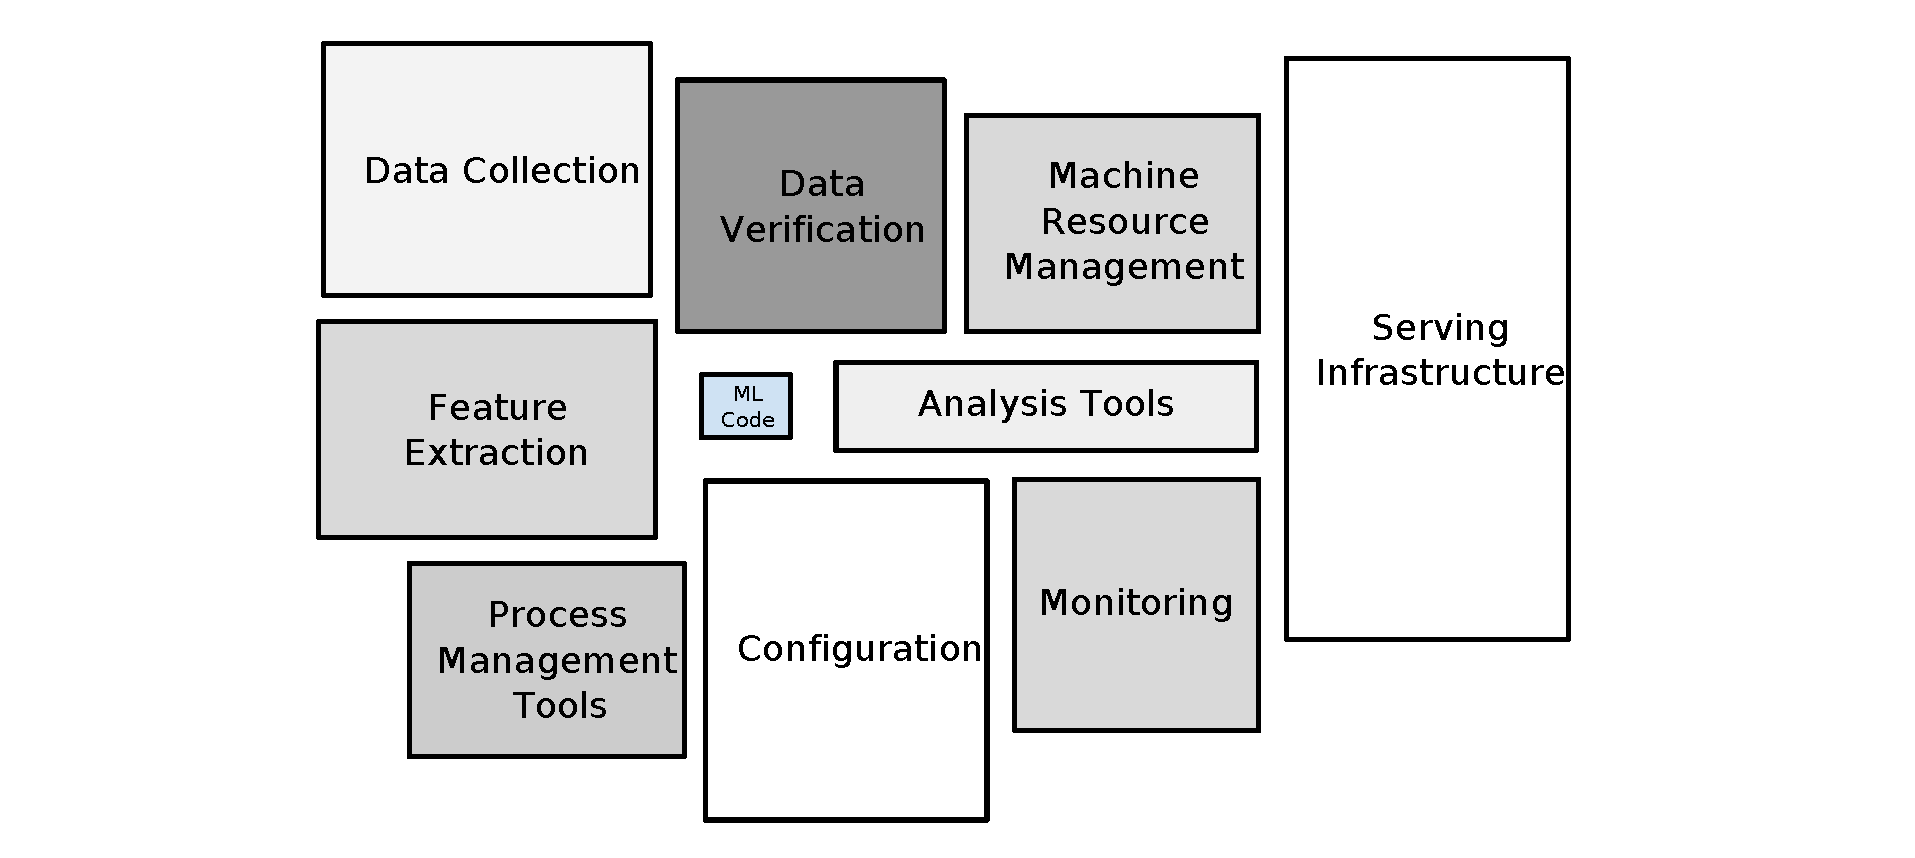
\includegraphics[width=.6\linewidth]{figures/MlSystem}
\end{center}
In the figure above, the box labeled \emph{ML Code} is the actual learning algorithm.  But in modern systems, this is but a small fraction of all of the tools needed to deploy a real world ML system.  This is not to say that we will be spending a lot of time learning about each of these other boxes (we will learn about some of them), but it helps to have a sense of the software echo system in which your ML model would be deployed.

\begin{quotation}
Also include the Alexa figure that Sam Daitzman found.
\end{quotation}

While it is helpful to remember that there are lots of other things in an ML system than just the core learning code, it is even more important to realize the \href{https://en.wikipedia.org/wiki/Sociotechnical_system}{socio-technical context} in which your system is deployed.  The figure above places the Amazon Echo within a larger environmental, social, and political context.  When designing and deploying systems, it will be necessary to consider the ways in which a developed solution might impact the world along these dimensions.

We'll be digging into some of these resources later in the course, but here are two papers that argue for the need to consider the development of ML systems from a socio-technical point of view.
\bi
\item \href{https://link.springer.com/article/10.1007/s11023-017-9417-6}{Reframing AI Discourse}
\item \href{https://dl.acm.org/citation.cfm?id=3287598}{Fairness and Abstraction in Sociotechnical Systems}
\ei


\subsection*{Idea 6: It's Not All Doom and Gloom}
While we'll be talking a lot about how ML can go wrong, unleashing unexpected consequences, we'll also be talking about the positive things that ML can do.  Here are just a couple of resources that discuss such systems (not to say that these systems don't have the potential to for things to go wrong).  We'll leave this list deliberately short to give you a chance to find your own example in the exercise below.

\bi
\item \href{https://www.springboard.com/blog/ai-for-good/}{AI for social good: 7 inspiring examples}
\item \href{https://medium.com/myplanet-musings/making-the-web-more-accessible-using-machine-learning-8a32eaafdb3a}{Machine Learning for Web Accessibility}
\ei


\marginnote{The \faShareAlt~icon means that will be submitting your response to this exercise with your assignment.  By default responses to exercises do not need to be submitted}

\begin{exercise}[\faShareAlt~(30 minutes)]
Now, we want to hear from you!  
\bes
\item Choose one of the big ideas above and write a short response to it.  Your response could incorporate something surprising you read, a thought-provoking question, your personal experience, an additional resource that builds upon or shifts the discussion.  We hope that this reflection will help scaffold class discussions and get you thinking about your interests in the big space that is ML.  Also, you have license from us to customize the structure of your response as you see fit.  As a rough guide, you should aim for a response of a 1-2 paragraphs.
\item Idea 6 talks about the idea of ML for positive impact.  What is one example of an ML application (real or imagined) that you think would have the largest (or most unambiguously) positive impact on the world?  Why?  Alternatively, what is an example of an ML application (real or imagined) that no matter how you carefully the designers approach it, should just not exist due to the harm it would cause the world?  Why?
\ees
\end{exercise}

\section{Mathematical Background}


\begin{notice}
For the purposes of this class, we will be consistent with the notation we use.  Of course, when we link to other resources, they may use other notation.  If notation is different in a way that causes confusion, we will try to point out pitfalls you should watch out for.  A guide to our notation conventions can be found on Canvas.  TODO: link out when we have this posted.
\end{notice}

\begin{externalresources}[(60 minutes)]
In order to engage with this assignment, you'll want to make sure you are familiar with the following concepts (links to resources embedded below):
\bi
\item Vector-vector multiplication
\bi
\item Section 2.1 of \href{https://see.stanford.edu/materials/aimlcs229/cs229-linalg.pdf}{Zico Kolter's Linear Algebra Review and Reference}
\ei
\item Matrix-vector multiplication
\bi
\item Section 2.2 of \href{https://see.stanford.edu/materials/aimlcs229/cs229-linalg.pdf}{Zico Kolter's Linear Algebra Review and Reference}
\item The first bits of the Khan academy video on \href{https://www.khanacademy.org/math/linear-algebra/matrix-transformations/linear-transformations/v/matrix-vector-products-as-linear-transformations}{Linear Transformations}
\ei
\item Partial derivatives and gradients
\bi
\item Khan Academy videos on partial derivatives: \href{https://www.khanacademy.org/math/multivariable-calculus/multivariable-derivatives/partial-derivatives/v/partial-derivatives-introduction}{intro}, \href{https://www.khanacademy.org/math/multivariable-calculus/multivariable-derivatives/partial-derivatives/v/partial-derivatives-and-graphs}{graphical understanding}, and \href{https://www.khanacademy.org/math/multivariable-calculus/multivariable-derivatives/partial-derivatives/v/formal-definition-of-partial-derivatives}{formal definition}
\item \href{https://www.khanacademy.org/math/multivariable-calculus/multivariable-derivatives/gradient-and-directional-derivatives/v/gradient}{Khan Academy video on Gradient}
\ei
\ei
\end{externalresources}

\begin{exercise}[(20 minutes)]
Here are some diagnostic problems to test some basic understanding of the concepts above.
\bes
\item Suppose $f(x, y) = 2x \sin{y} + y^2 x$.  Calculate $\frac{\partial{f}}{\partial{x}}$, $\frac{\partial{f}}{\partial{x}}$, and $\nabla f$.
\item Suppose $\mlvec{x} = \begin{bmatrix} 3 \\ -1 \\ 4 \end{bmatrix}$ and $\mlvec{y} = \begin{bmatrix} 2 \\  7 \\ 4 \end{bmatrix}$.  Calculate $\mlvec{x} \cdot \mlvec{y}$, $\mlvec{x}^\top \mlvec{y}$, and $\mlvec{x} \mlvec{y}^\top$.
\item Let $\mlmat{A} = \begin{bmatrix} \mlvec{col_1} & \mlvec{col_2} & \ldots & \mlvec{col_n} \end{bmatrix} = \begin{bmatrix} \mlvec{row_1}^\top \\ \mlvec{row_2}^\top \\ \vdots \\ \mlvec{row}_m^\top \end{bmatrix}$

(that is, the matrix $\mlmat{A}$ can either be thought of as consisting of the columns $\mlvec{col_1}, \ldots, \mlvec{col_n}$ or the rows $\mlvec{row_1}^\top, \ldots, \mlvec{row_m}^\top$).

Compute $\mlmat{A}\mlvec{v}$ in terms of $\mlvec{col_1}, \ldots, \mlvec{col_n}$.

Compute $\mlmat{A} \mlvec{v}$ in terms of the rows of $\mlvec{row_1}, \ldots, \mlvec{row_m}$.
\ees
\end{exercise}

\section{Linear Regression from the Top-Down}

\subsection*{Motivation: Why Learn About Linear Regression?}
Before we jump into the \emph{what} of linear regression, let's spend a little bit of time talking about the \emph{why} of linear regression.  As you'll soon see, linear regression is among the simplest (perhaps \emph{the} simplest) machine learning algorithm.  It has many limitations, which you'll also see, but also a of ton strengths.  \textbf{First, it is a great place to start when learning about machine learning} since the algorithm can be understood and implemented using a relatively small number of mathematical ideas (you'll be reviewing these ideas later in this assignment).  In terms of the algorithm itself, it has the following very nice properties.

\bi
\item \textbf{Transparent:} it's pretty easy to examine the model and understand how it arrives at its predictions.
\item \textbf{Computational tractable:} linear regression models can be trained efficiently on datasets with large numbers of features and data points.
\item \textbf{Easy to implement:} linear regression can be implemented using a number of different algorithms (e.g., gradient descent, closed-form solution).  Even if the algorithm is not built into your favorite numerical computation library, the algorithm can be implemented in only a couple of lines of code.
\ei


For linear regression we assume that our input points, $\mlvec{x_i}$, are d-dimensional vectors (each entry of these vectors can be though of as a feature), that our output points, $y_i$, are scalars, and that our prediction functions $\hat{f}$ are all of the form $\hat{f}(\mlvec{x}) = \mlvec{w}^\top \mlvec{x} = \sum_{i=1}^d w_i x_i$ for some vector of weights $\mlvec{w}$ (you could think of $\hat{f}$ as also taking $\mlvec{w}$ as an input, e.g., writing $\hat{f}(\mlvec{x}, \mlvec{w}$).  When it's obvious what the value of $\mlvec{w}$ is, we'll leave it as an implicit input instead, e.g., writing $\hat{f}(\mlvec{x})$).

In the function, $\hat{f}$, the elements of the vector $\mlvec{w}$ represent weights that multiply various entries of the input.  For instance, if an element of $\mlvec{w}$ is high, that means that as the corresponding element of $\mlvec{x}$ increases, the prediction that $\hat{f}$ generates for $\mlvec{x}$ would also increase (you may want to mentally think through other cases, e.g., what would happen is the element of $\mlvec{x}$ decreases, or what would happen if the entry of $\mlvec{w}$ was large and negative).  The products of the weights and the features are then summed to arrive at an overall prediction.

Given this model, we can now define our very first machine learning algorithm: \href{https://en.wikipedia.org/wiki/Ordinary_least_squares}{ordinary least squares} (OLS)!  In the ordinary least squares algorithm, we use our training set to select the $\mlvec{w}$ that minimizes the sum of squared differences between the model's predictions and the training outputs.  Thinking back to the supervised learning problem setup, this corresponds to choosing $\ell(y, \hat{y}) = (y - \hat{y})^2$.
Therefore, the OLS algorithm will use the training data to select the optimal value of $\mlvec{w}$ (called $\mlvec{w}^\star$), which minimizes the sum of squared differences between the model's predictions and the training outputs.

\begin{align}
\mlvec{w}^\star &= \argmin_{\mlvec{w}} \sum_{i=1}^n \ell \left ( \hat{f}(\mlvec{x_i}, \mlvec{w}) , y_i \right) \\
\mlvec{w}^\star &= \argmin_{\mlvec{w}} \sum_{i=1}^n \left ( \hat{f}(\mlvec{x_i}, \mlvec{w}) - y_i \right)^2 \\
&= \arg\min_{\mlvec{w}} \sum_{i=1}^n \left ( \mlvec{w}^\top \mlvec{x_i} - y_i \right)^2
\end{align}

While we haven't talked at all about how to find $\mlvec{w}^\star$, that will be the focus of a later part of this assignment, once we have $\mlvec{w}^\star$ we can predict a value for a new testing point, $\mlvec{x}$, by predicting that the corresponding (unknown) label, $y$, as $\hat{y} = \mlvec{w}^\top \mlvec{x}$.  In this way, we have used the training data to learn how to make predictions about unseen data points, which is the hallmark of supervised machine learning!

\begin{exercise}
Draw a scatter plot in 2D (the x-axis is the independent variable and the y-axis is the dependent variable).  Fill in a few datapoints and draw a potential line of best fit.  On the plot identify the differences between the data points and the line (these differences are the residuals).  Draw a second potential line of best fit and mark the residuals.  From the point of view of ordinary least-squares, which of these lines is better.
\end{exercise}

\section{Getting a Feel for Linear Regression}
In this class we'll be learning about algorithms using both a top-down and a bottom-up approach.  By bottom-up we mean applying various mathematical rules to derive a solution to a problem and only then trying to understand how to apply it and how it well it might work for various problems.  By top-down we mean starting by applying the algorithm to various problems and through these applications gaining a sense of the algorithm's properties before learning how to derive / implement it.  We'll start our investigation of linear regression using a \textbf{top-down approach}.


\subsection{Linear Regression with One Input Variable: Line of Best Fit}
If any of what we've said so far sounds familiar, it is likely because you have seen the idea of a line of best fit in some previous class.  To understand more intuitively what the OLS algorithm is doing, we want you to investigate its behavior when there is a single input variable (i.e., you are computing a line of best fit).  

\begin{externalresources}
Use the \href{http://www.shodor.org/interactivate/activities/Regression/}{line of best fit online app} to create some datasets, guess the line of best fit, and then compare the results to the OLS solution.

\begin{exercise}
\bes
\item Examine the role that outliers play in determining the line of best fit.  Does OLS seem sensitive or insensitive to the presence of outliers in the data?
\item Were there any times when the line of best fit didn't seem to really be ``best'' (e.g., it didn't seem to capture the linear trends in the data)?
\ees
\end{exercise}

\end{externalresources}



\subsection{Linear Regression with Multiple Input Variables: Explorations in Python}
\begin{externalresources}[(90 minutes)]
Work through the \href{https://colab.research.google.com/drive/12pLbQkhrPoI-22FVV6gZNObi1IJCW-mF}{Assignment 1 Companion Notebook} to get some practice with {\tt numpy} and explore linear regression using a top-down approach.  You can place your answers directly in the Jupyter notebook so that you have them for your records.

\end{externalresources}



\end{document}
